%%%%%%%%%%%%%%%%%%%%%%%%%%%%%%%%%%%%%%%%%%%%%%%%%%%%%%%%%%%%%%%%%%%%%%%%%%%

\documentclass{standalone}

\usepackage{mathptmx}
\usepackage{tikz}
\usetikzlibrary{external}
\tikzexternalize{quadrant}

%% We default to Times.
\renewcommand{\rmdefault}{ptm}
\renewcommand{\ttdefault}{pcr}
%% Enable Times/Palatino main text font.
\normalfont\selectfont

\newcommand{\comma}{,\,}
\newcommand{\tuple}[2]{\left( {#1}\comma {#2} \right)}

%% A quadrant of the unit circle.
\newcommand{\myQuadrant}{%%
  %% Draw the quadrant.
  \draw[lineStyle] (A) arc (\angleStart:\angleEnd:\radius) -- (origin)
  -- cycle;
  %% Label the origin.
  \node[nodeStyle] at (origin) {};
  \node at (origin) [below] {$\tuple{0}{0}$};
}

%% A quarter of a polygon inscribed within a quadrant of the unit
%% circle.
\newcommand{\myPolygon}{%%
  %% Draw the inscribed square.
  \draw[lineStyle] (A) -- (B) -- (C) -- (D) -- (E);
  % %% Label the points where the circle meet the polygon.
  %% Point A.
  \node[nodeStyle] at (A) {};
  \node at (A) [right] {$A = \tuple{1}{0}$};
  %% Point B.
  \node[nodeStyle] at (B) {};
  \node at (B) [right]
  {$B = \tuple{\frac{\sqrt{2 + \sqrt{2}}}{2}}{\frac{\sqrt{2 - \sqrt{2}}}{2}}$};
  %% Point C.
  \node[nodeStyle] at (C) {};
  %% Point D.
  \node[nodeStyle] at (D) {};
  %% Point E.
  \node[nodeStyle] at (E) {};
}

%% Approximating pi with an inscribed polygon.

\begin{document}

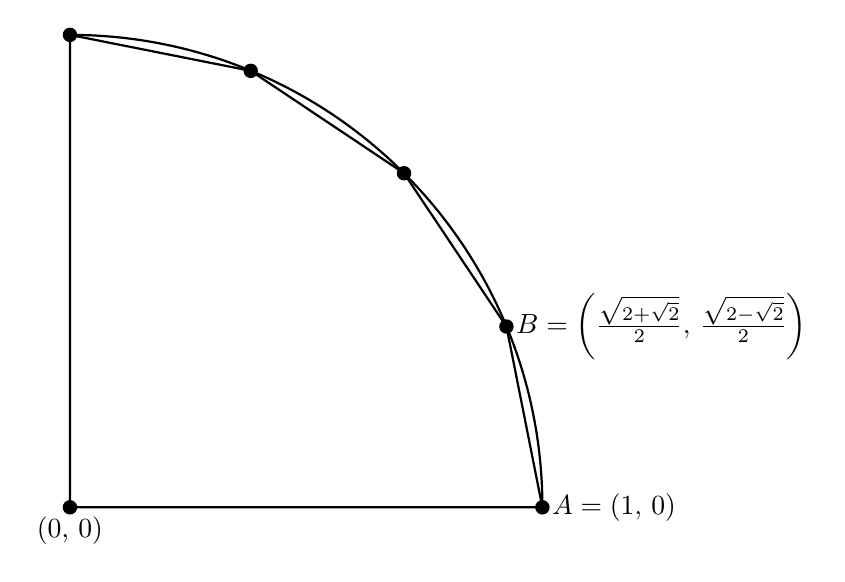
\begin{tikzpicture}[%%
  lineStyle/.style={-,thick},%%
  nodeStyle/.style={draw,inner sep=1.7pt,circle,fill=black,black}
]
%%
%%
%% The quadrant.
\pgfmathsetmacro{\angleEnd}{90}   %% angle in degrees
\pgfmathsetmacro{\angleStart}{0}  %% angle in degrees
\pgfmathsetmacro{\radius}{6}
%%
\pgfmathsetmacro{\xlow}{0}
\pgfmathsetmacro{\ylow}{\xlow}
%%
\coordinate (origin) at (\xlow,\ylow);
%% Coordinates of where the polygon touches the circle.
\coordinate (A) at (\xlow+\radius,\ylow);
\coordinate (B) at (5.54327719506772,2.29610059419054);
\coordinate (C) at (4.24264068711929,4.24264068711929);
\coordinate (D) at (2.29610059419054,5.54327719506772);
\coordinate (E) at (\xlow,\ylow+\radius);
%%
%% Draw a circle with an inscribed polygon.
\myQuadrant
\myPolygon
\end{tikzpicture}

\end{document}
